\documentclass{article}
\usepackage[utf8]{inputenc}
\usepackage[T1]{fontenc}
\usepackage{graphicx}
\usepackage{enumerate}
\renewcommand{\contentsname}{Sadržaj}
\begin{document}



\begin{titlepage}

\newcommand{\HRule}{\rule{\linewidth}{0.5mm}} 

\center 


\textsc{\LARGE Univerzitet u Beogradu\\ Matematički Fakultet }\\[1.5cm] 
\textsc{\Large Informacioni sistemi}\\[0.5cm] 
\textsc{\large Grupni sudentski rad}\\[0.5cm] 



\HRule \\[0.4cm]
{ \huge \bfseries Informacioni sistem ugostiteljskog objekta}\\[0.4cm] 
\HRule \\[1.5cm]
 


\begin{minipage}{0.4\textwidth}
\begin{flushleft} \large
\emph{Mentori:}\\
Dr. Saša Malkov\\
Aleksandra Kocić
\end{flushleft}
\end{minipage}
~
\begin{minipage}{0.4\textwidth}
\begin{flushright} \large
\emph{Studenti:} \\
Aleksandra Branković \\
Jasmina Vasilijević\\
Sanela Numanović\\
Božidar Radivojević\\
Miloš Šuković\\
\end{flushright}
\end{minipage}\\[2cm]


 
{\large Beograd,\\ decembar 2017.}\\[2cm] 

\includegraphics[width=3cm,height=3cm, keepaspectratio]{matf.jpg}\\[1cm]
 

\vfill 

\end{titlepage}

\tableofcontents
\newpage
%%%%%%%%%%%%%%%%%%%%%%%%%%%%%%%%%%%%%%%%%%%%%%%%%%%%%%%%%%%%%%%%%%%%%%%%%%%%

\section{Uvod}
\emph{Najmanji Problem} je ime izmišljenog ugostiteljskog objekta (kafe/klub/restoran) u Beogradu, za koji treba konstruisati informacioni sistem, u cilju maksimizovanja profita, kroz smanjenje troškova i povećanje transparentnosti
poslovanja.\\


Rad je izrađen kao grupni studentski projekat na Matematičkom fakultetu, na studijskom programu Računarstvo i informatika,  Master studije. Projekat je odrađen pod nadzorom profesora dr. Saše Malkova i asistentkinje Aleksandre Kostić, u okviru predmeta Informacioni sistemi.\\


%%%%%%%%%%%%%%%%%%%%%%%%%%%%%%%%%%%%%%%%%%%%%%%%%%%%%%%%%%%%%%%%%%%%%%%%%%%%



\subsection{Metodologija rada}

Celina sistema, kao i uočene grupe poslova unutar istog, analizirani su dijagramima slučajeva upotrebe. Pojedine uočene celine detaljnije su modelirane BPMN (Business Process Modelling Notation) dijagramima. Za izdradu baze podataka upotrebljen je ER dijagram.

%%%%%%%%%%%%%%%%%%%%%%%%%%%%%%%%%%%%%%%%%%%%%%%%%%%%%%%%%%%%%%%%%%%%%%%%%%%%

\subsection{Korišćeni alati}
Za izdradu dijagrama slučajeva upotrebe i ER dijagrama :
\begin{itemize}
\item Visual Paradigm for UML
\end{itemize}
Za izradu BPMN dijagrama :
\begin{itemize}
\item Modelio
\end{itemize}
Nacrt korisničkog interfejsa :
\begin{itemize}
\item Balsamiq 3.0
\end{itemize}

%%%%%%%%%%%%%%%%%%%%%%%%%%%%%%%%%%%%%%%%%%%%%%%%%%%%%%%%%%%%%%%%%%%%%%%%%%%%
\section{Analiza sistema}

Moderni ugostiteljski objekti postaju sve više zavisni od informacionih tehnologija u svakodnevnom radu, dok su sa druge strane čvrsto vezani i za zastarele oblike komunikacije i rada ukorenjene u lokalnim običajima, čineći specifičnu
mešavinu dva sveta.\\

Vođenje ugostiteljskih objekata uključuje niz aktivnosti, čije izvršavanje može biti olakšano, ubrzano i učinjeno transparentnom implementacijom digitalnog informacionog sistema, koji bi obezbeđivao sledeće funkcionalnosti:\\

\begin{itemize}
\item Pregled stanja zaliha namirnica i druge potrošne robe u realnom vremenu
\item Pregled inventara pribora, nameštaja i uređaja neophodnih za funkcionisanje objekta
\item Pregled finansijskog stanja, ulaza i izlaza, kreiranje finansijskih izveštaja
\item Upravljanje ljudskim resursima (raspored godišnjih odmora, raspored smena)
\item Prihvatanje rezervacija gostiju
\item Online naručivanje i dostava hrane i pića
\item Pregled stanja trenutno aktivnih narudžbina (fizičkih i online), i razmena informacija između konobara i kuhinje
\end{itemize}

Neki od podsistema su otvoreni, a neki zatvoreni, tako da postoji mogućnost demonstracije različitih tehnika razvoja
informacionih podsistema.\\

Problematika realnog sistema na kojem treba da počiva ovaj informacioni sistem je svima poznata u dovoljnoj meri, da je moguće izvršiti inicijalno planiranje u grubim crtama, dok je za detaljniji plan neophodno terensko istraživanje.\\

Krajnji rezultat ovog projekta jeste funkcionalni prototip informacionog sistema.\\

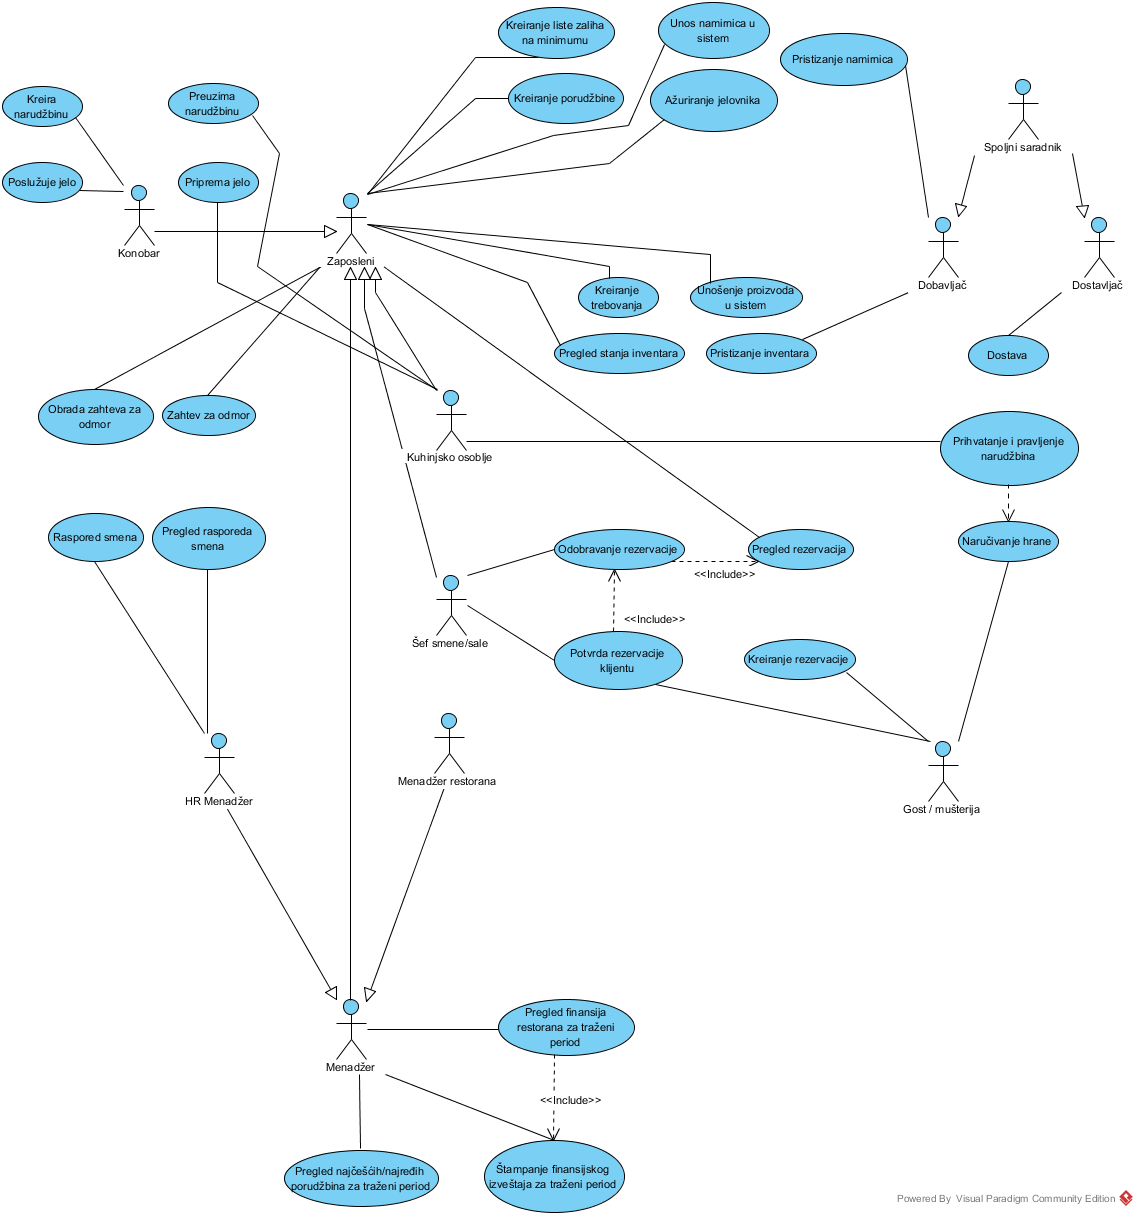
\includegraphics[width=\textwidth]{SU_0_grupni.png}


\section{Slučajevi upotrebe}


Slučaj upotrebe (Use case) je specifikacija skupa akcija koje vrši sistem, koje proizvode vidljiv rezultat koji je, po pravilu, od vrednosti za jednog ili više učesnika u sistemu. Koristi se da precizira ponašanje sistema, bez otkrivanja njegove unutrašnje strukture.


%%%%%%%%%%%%%%%%%%%%%%%%%%%%%%%%%%%%%%%%%%%%%%%%%%%%%%%%%%%%%%%%%%%%%%%%%%%%

\subsection{Zalihe namirnica}
Pregled stanja zaliha namirnica je slučaj upotrebe u kome se formalizuje način na koji ugostiteljski objekat planira nabavku namirnica, nabavlja, a potom ih dodaje na stanje. U tom procesu učestvuju menadžer nabavke (zaposleni) i dobavljač. 

\begin{itemize}
\item Zaposleni kreira spisak namirnica čija je trenutna količina ispod propisane minimalne. Na osnovu tog spiska, kreira porudžbinu. Kasnije, nakon isporuke porudžbine, unosi u bazu pristiglu robu.
\item Dobavljač isporučuje ugostiteljskom objektu namirnice u traženoj količini.
\end{itemize}
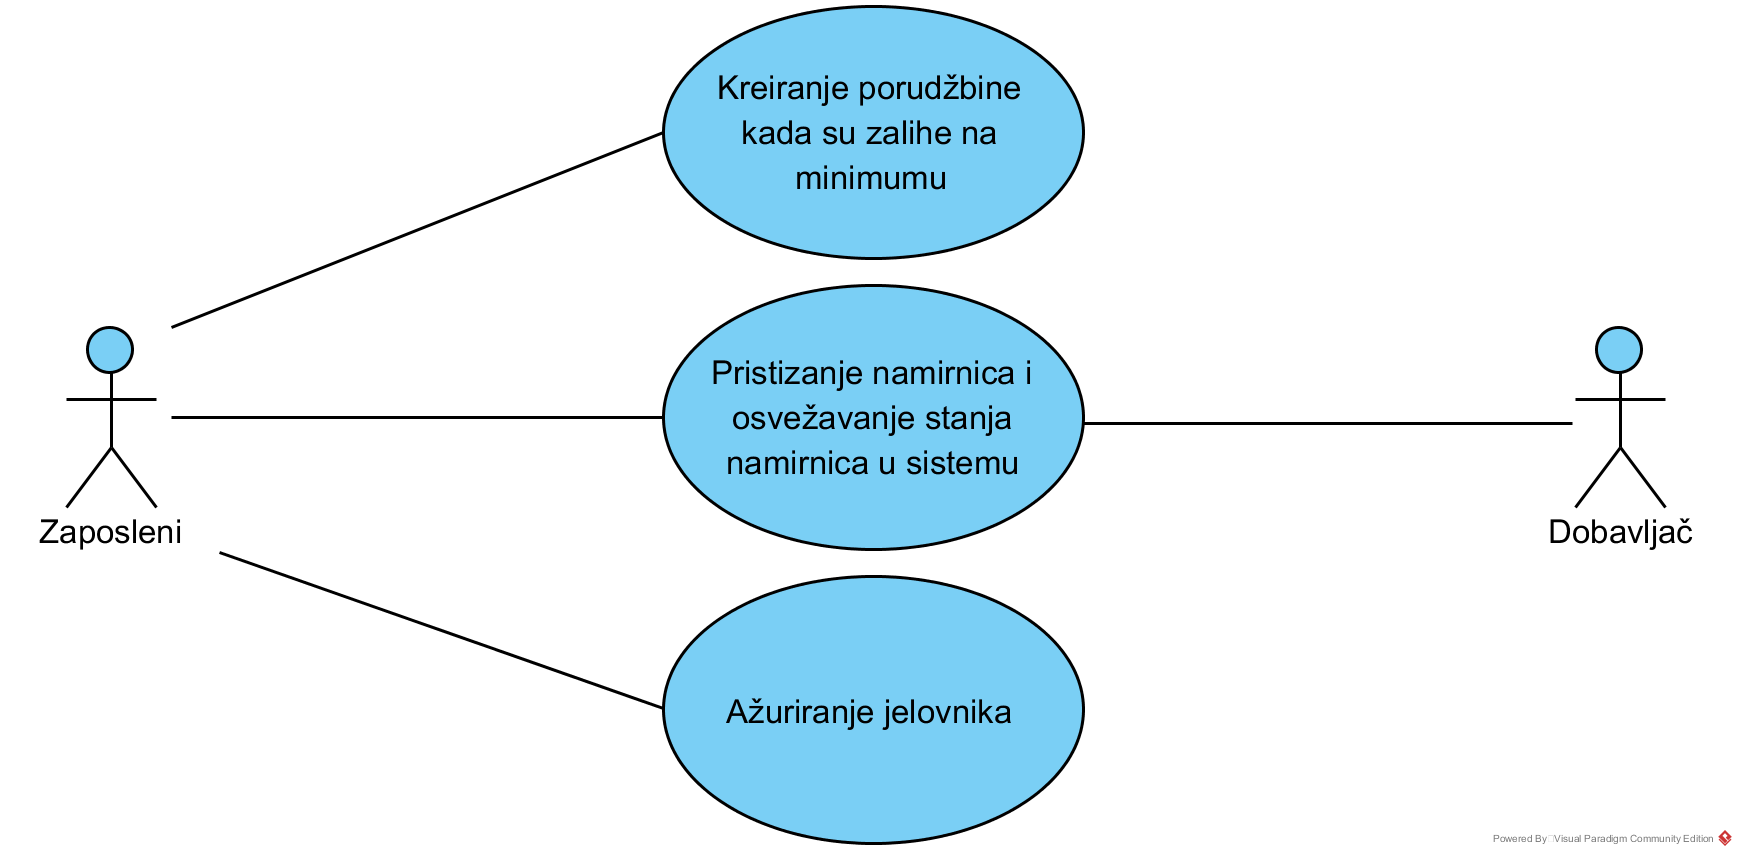
\includegraphics[width=\textwidth]{SU_1_zalihe.png}
\subsubsection{\textbf{Use Case}: Zalihe na minimumu}
\textbf{Akter:} Radnik/menadžer nabavke\\
\textbf{Ulaz:} Nema\\
\textbf{Izlaz:} Kreiran je spisak namirnica čije su zalihe na minimumu.\\
\textbf{Preduslovi:} Radnik poseduje username i lozinku za prijavljivanje na glavni sistem gde se nalaze informacije o namirnicama.\\
\textbf{Postuslov:} Uspešno je kreiran spisak namirnica.\\
\textbf{Glavni tok:} 
\begin{enumerate}
	\item Radnik se prijavljuje na sistem.
	\item Radnik zahteva od sistema spisak namirnica za koje važi da je trenutna količina manja od minimalne propisane.
	\item Sistem generiše listu namirnica koje zadovoljavaju prethodno navedeni uslov.
\end{enumerate}
\textbf{Alternativni tokovi:} \\
\begin{itemize}
\item [1.1.] Prijavljivanje nije uspešno, korisnik se preusmerava na poruku sa greškom.
\item[2.1] Ukoliko ne postoji ni jedan proizvod koji ima definisanu minimalnu količinu, izveštaj o zalihama na minimumu se ne može generisati.
\end{itemize}
	 

\subsubsection{\textbf{Use Case}: Kreiranje porudžbine}
\textbf{Akter:} Radnik/menadžer nabavke\\
\textbf{Ulaz:} Lista namirnica čije su zalihe na minimumu.\\
\textbf{Izlaz:} Lista poručenih namirnica.\\
\textbf{Preduslovi:} Ranik se uspešno prijavio na sistem i ima uvid u spisak namirnica čija je količina manja od poželjne.\\
\textbf{Postuslov:} Porudžbina je kreirana.\\
\textbf{Glavni tok:} 
\begin{enumerate}
	\item Radnik uzima listu namirnica koje bi trebalo nabaviti.
	\item Za svaku namirnicu procenjuje količinu za nabavku. 
	\item Na spisak može dodati i namirnice kojih nema i nikada ih nije bilo u sistemu. 
	\item Kreira porudžbinu.
\end{enumerate}
\textbf{Alternativni tokovi:}
\begin{itemize}
\item[1.1] Ukoliko je lista namirnica na minimalnim zalihama prazna, procena se ne vrši. 
\end{itemize}

\subsubsection{\textbf{Use Case}:  Pristizanje namirnica}
\textbf{Akter:} Dobavljač\\
\textbf{Ulaz:} Lista poručenih namirnica.\\
\textbf{Izlaz:} Lista namirnica koje je dobavljač isporučio ugostiteljskom objektu.\\
\textbf{Preduslovi:} Dobavljač je dobio porudžbinu.\\
\textbf{Postuslov:} Namirnice su isporučene kupcu i kreirana je lista dostavljenih proizvoda.\\
\textbf{Glavni tok:} 
\begin{enumerate}
	\item Dobavljač je primio porudžbinu.
	\item Procenjuje da li je njegva firma u mogućnosti da odgovori na zahteve ugostiteljskog objekta.
	\item Za svaku namirnicu odlučuje da li će isporučiti u smanjenoj ili traženoj količini.
	\item Isporučuje robu ugostiteljskom objektu.
	\item Pri isporuci dostavljena je lista namirnica koje su isporučene.
\end{enumerate}
\textbf{Alternativni tokovi:} 
\begin{itemize}
\item[2.1.] Zbog manjka raspoloživih namirnica, dobavljač otkazuje porudžbinu.
\end{itemize}


\subsubsection{\textbf{Use Case}: Unos namirnica u sistem}
\textbf{Akter:} Radnik\\
\textbf{Ulaz:} Spisak namirnica koje je dobavljač isporučio.\\
\textbf{Izlaz:} Ažurirana je lista namirnica.\\
\textbf{Preduslovi:} Radnik se uspešno prijavio na sistem. Dobavljač je dostavio poručene namirnice.\\
\textbf{Postuslov:} Ažurirane su količine namirnica i eventualno unete nove.\\
\textbf{Glavni tok:} 
\begin{enumerate}
	\item Radnik je dobio listu isporučenih namirnica.
	\item Za svaki od proizvoda sa liste, radnik ažurira proizvod u sistemu tako što dodaje pristiglu količinu.
	\item Ukoliko proizvod ne postoji u sistemu, radnik kreira novi.
	\item Ažurira novokreiranu namirnicu pristiglom količinom i eventualno definiše minimalnu količinu. 
\end{enumerate}
\textbf{Alternativni tokovi:}
\begin{itemize}
\item [1.1.] Porudžbina je otkazana od strane dobavljača, nema unosa.
\end{itemize}


\subsubsection{\textbf{Use Case}: Ažuriranje jelovnika}
\textbf{Akter:} Radnik\\
\textbf{Ulaz:} Spisak namirnica u restoranu i spisak jela sa neophodnim namirnicama za njihovu pripremu.\\
\textbf{Izlaz:} Kreiran je jelovnik.\\
\textbf{Preduslovi:} Radnik se uspešno prijavio na sistem. Spisak jela i sastojaka od kojih se pripremaju nije prazan.\\
\textbf{Postuslov:} Jelovnik je kreiran. Gosti i zaposleni ga mogu videti.\\
\textbf{Glavni tok:} 
\begin{enumerate}
	\item Radnik zahteva od sistema ažuriranje jelovnika.
	\item Sistem na njegov zahtev kreira novi jelovnik tako što iz liste jela izbacuje ona za čiju pripremu nedostaje makar jedan sastojak.
	\item Kreirani jelovnik postaje aktuelni jelovnik ugostiteljskog objekta.
\end{enumerate}
\textbf{Alternativni tokovi:}
\begin{itemize}
\item [1.1] Ne postoje podaci koji povezuju jela i namirnice, novi jelovnik se ne može generisati. Aktuelni jelovnik se ne ažurira.
\end{itemize}

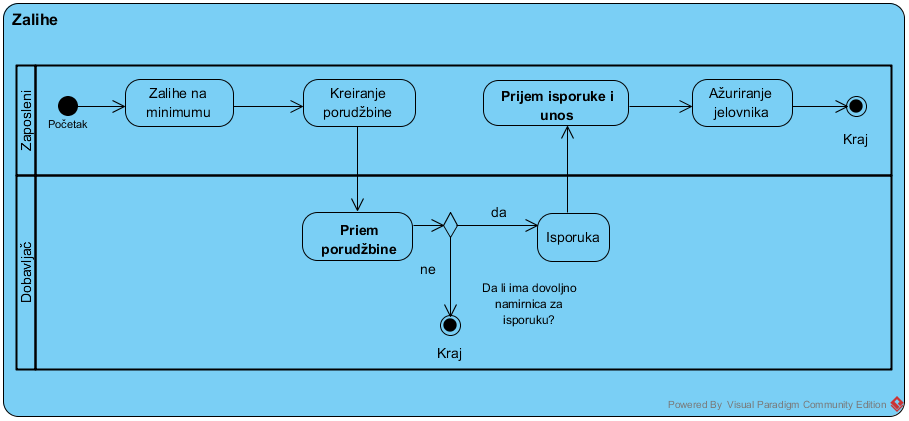
\includegraphics[width=\textwidth]{SU_1_zalihe_activity.png}

%%%%%%%%%%%%%%%%%%%%%%%%%%%%%%%%%%%%%%%%%%%%%%%%%%%%%%%%%%%%%%%%%%%%%%%%%%%%

\subsection{Pregled inventara}
Pregled inventara je slučaj upotrebe u kome se formalizuje način na koji ugostiteljski objekat planira nabavku inventara, nabavlja i ima uvid o stanju istog. U tom procesu učestvuju radnik i dobavljač. 

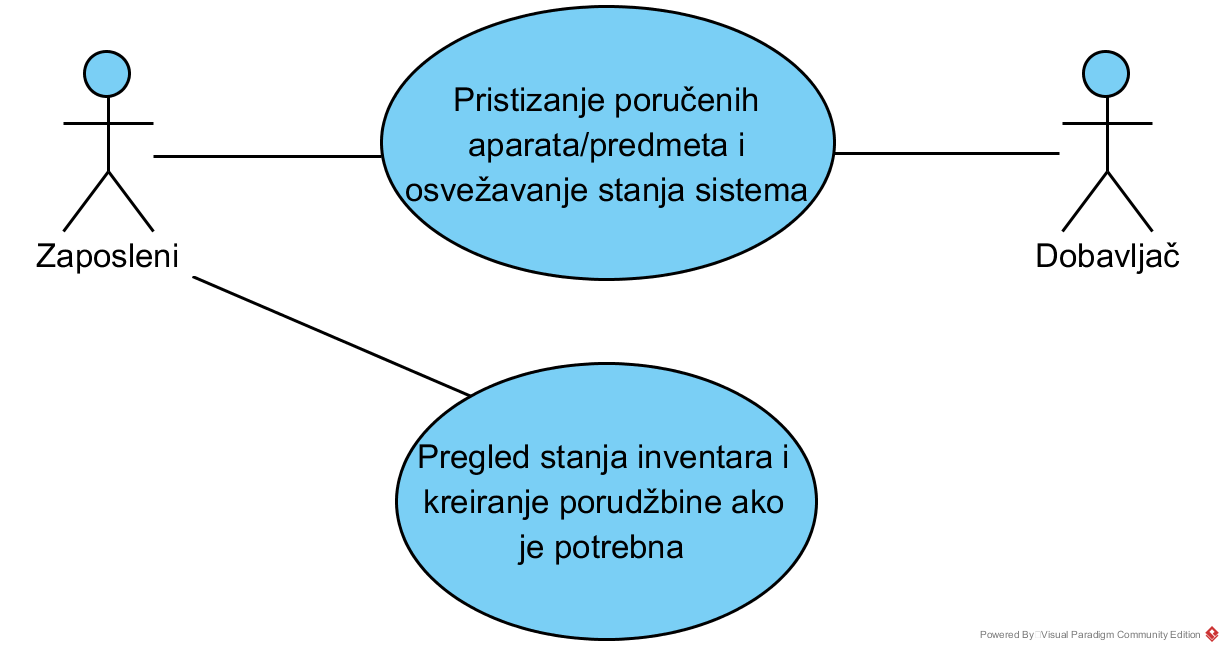
\includegraphics[width=\textwidth]{SU_2_pregled_inventara.png}
\subsubsection{\textbf{Use Case}: Pregled stanja inventara}
\textbf{Akter:} Zaposleni restorana\\
\textbf{Ulaz:} Nema\\
\textbf{Izlaz:} 
\begin{enumerate}
	\item Spisak predmeta koji spadaju u inventar ugostiteljskog objekta i njihove zalihe su usled kvara ili nestanka ispod minimalnih definisanih količina.
	\item Lista svih predmeta i njihova trenutna količina.
\end{enumerate} 
\textbf{Preduslovi:} Radnik se uspešno ulogovao na sistem.\\
\textbf{Postuslov:} Uspešno je kreiran spisak predmeta. Ukoliko neki predmet zahteva popravku, lista sadrži tu informaciju.\\
\textbf{Glavni tok:} 
\begin{enumerate}
	\item Radnik zahteva od sistema spisak predmeta za koje važi da je trenutna količina manja od minimalne propisane ili je neki od aparata u kvaru.
	\item Sistem kreira listu predmeta koji ispunjavaju prethodni zahtev.
\end{enumerate}
\textbf{Alternativni tokovi:}
\begin{itemize}
\item [1.1] Ne postoje podaci o minimalnim količinama ni za jedan predmet u sistemu, pa nije moguće kreirati pregled stanja.
\end{itemize}

\subsubsection{\textbf{Use Case}: Kreiranje porudžbine}
\textbf{Akter:} Zaposleni restorana\\
\textbf{Ulaz:} Lista predmeta čije su zalihe ispod minimalnih definisanih za poslovanje ugostiteljskog objekta.\\
\textbf{Izlaz:} Lista poručenih predmeta.\\
\textbf{Preduslovi:} Radnik je uspešno ulogovan i ima uvid u spisak predmeta čija je količina manja od poželjne.\\
\textbf{Postuslov:} Porudžbina je kreirana.\\
\textbf{Glavni tok:} 
\begin{enumerate}
	\item Radnik uzima listu predmeta koje bi trebalo nabaviti.
	\item Radnik procenjuje količinu za nabavku. 
	\item Radnik proverava da li postoje predmeti koje želi da uvrsti u inventar i doda ih u porudžbinu.
	\item Kreira porudžbinu.
\end{enumerate}
\textbf{Alternativni tokovi:} 
\begin{itemize}
\item [1.1] Ukoliko je lista predmeta na minimalnim zalihama prazna, procena količina se ne vrši.
\end{itemize}

\subsubsection{\textbf{Use Case}:  Pristizanje predmeta i aparata}
\textbf{Akter:} Dobavljač\\
\textbf{Ulaz:} Lista poručenih predmeta.\\
\textbf{Izlaz:} Lista predmeta koje je dobavljač isporučio ugostiteljskom objektu.\\
\textbf{Preduslovi:} Dobavljač je dobio porudžbinu.\\
\textbf{Postuslov:} Predmeti su isporučeni kupcu i kreirana je lista dostavljenih proizvoda.\\
\textbf{Glavni tok:} 
\begin{enumerate}
	\item Dobavljač je dobio listu poručenih proizvoda.
	\item Proverava za svaki proizvod da li je njegova firma u mogućnosti da isporuči tražene količine.
	\item Po potrebi, smanjuje količine koje su poručene.
	\item Isporučuje robu ugostiteljskom objektu.
	\item Pri isporuci dostavljena je lista predmeta koji su isporučeni.
\end{enumerate}
\textbf{Alternativni tokovi:} 
\begin{itemize}
\item [2.1] Zbog manjka raspoloživih predmeta, dobavljač otkazuje porudžbinu.
\end{itemize}


\subsubsection{\textbf{Use Case}: Unos predmeta u sistem}
\textbf{Akter:} Radnik\\
\textbf{Ulaz:} Spisak predmeta koje je dobavljač isporučio.\\
\textbf{Izlaz:} Ažurirana je lista predmeta koji čine inventar.\\
\textbf{Preduslovi:} Radnik se uspešno ulogovao na sistem. Dobavljač je dostavio poručene proizvode.\\
\textbf{Postuslov:} Ažurirane su količine proizvoda i eventualno uneti novi.\\
\textbf{Glavni tok:} 

\begin{enumerate}
	\item Radnik je dobio listu isporučenih proizvoda.
	\item Za svaki od proizvoda sa liste, radnik ažurira proizvod u sistemu tako što dodaje pristiglu količinu.
	\item Ukoliko proizvod ne postoji u sistemu, radnik kreira proizvod sa njegovim karakteristikama.
	\item Ažurira novokreirani proizvod pristiglom količinom i eventualno definiše minimalnu količinu. 
\end{enumerate}
\textbf{Alternativni tokovi:} 
\begin{itemize}
\item [1.1] Porudžbina je otkazana, nema unosa.
\end{itemize}

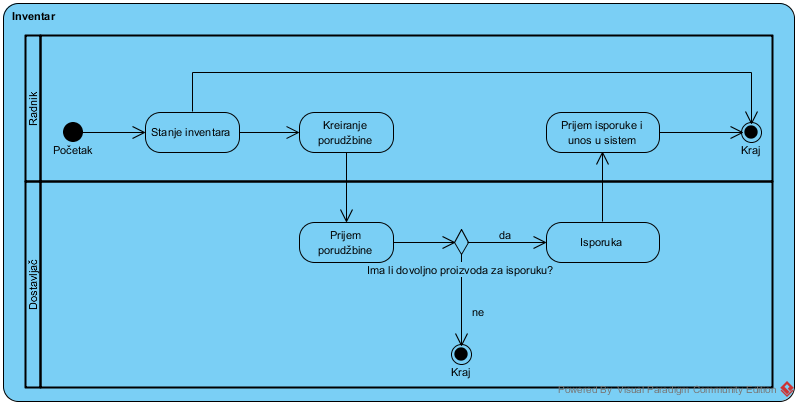
\includegraphics[width=\textwidth]{SU_2_pregled_inventara_activity.png}

%%%%%%%%%%%%%%%%%%%%%%%%%%%%%%%%%%%%%%%%%%%%%%%%%%%%%%%%%%%%%%%%%%%%%%%%%%%%

\subsection{Pregled finansijskog stanja}
Pregled finansijskog stanja je slučaj upotrebe u kojem menadžer restorana ima mogućnost pregleda prihoda i rashoda za dati vremenski period, koji se izračunavaju na osnovu naplaćenih usluga i troškova nabavke, održavanja, prihoda zaposlenih, itd.
\\
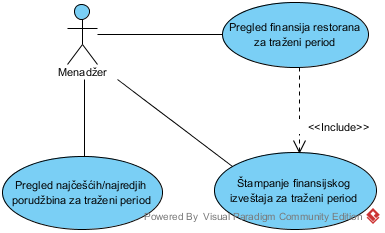
\includegraphics[width=\linewidth]{SU_3_pregled_finansija.png}

\subsubsection{\textbf{Use Case}: Pregled finansija restorana za traženi period}
\textbf{Akter:} Menadžer\\
\textbf{Ulaz:} Datum početka perioda od interesa, datum kraja perioda od interesa\\
\textbf{Izlaz:} Tabelarni prikaz prihoda i rashoda za traženi period\\
\textbf{Preduslovi:} Menadžer ima pravo pristupa stranici za pregled finansija.\\
\textbf{Postuslov:} Nema\\
\textbf{Glavni tok:}
\begin{enumerate}
\item Korisnik se prijavljuje na sistem
\item Korisnik vrši odabir početnog i krajnjeg dana perioda od interesa
\item Korisnik dobija spisak prihoda i rashoda u datom vremenskom periodu.
\end{enumerate}
\textbf{Alternativni tokovi:} \\
\begin{itemize}
\item [1.1.] Prijavljivanje nije uspešno, korisnik se preusmerava na poruku sa greškom.
\item [2.1.] Uneti datumi nisu validni, korisnik se moli da ponovo unese datume i nastavlja ka koraku 3.\\
\item [3.1.] Za unete datume, restoran nije imao nijedan poslovni dan, prikazuje se adekvatna poruka na ekranu i korisnik se preusmerava nazad na 2. korak
\end{itemize}
        
		
\subsubsection{\textbf{Use Case}: Štampanje finansijskog izveštaja za traženi period}
\textbf{Akter:} Menadžer\\
\textbf{Ulaz:} Datum početka perioda od interesa, datum kraja perioda od interesa, način štampanja.\\
\textbf{Izlaz:} Tabelarni prikaz prihoda i rashoda za traženi period i .pdf verzija finansijskog izveštaja.\\
\textbf{Preduslovi:} Menadžer ima pravo pristupa stranici za pregled finansija.\\
\textbf{Postuslov:} Odštampan finansijski izveštaj ima identične podatke kao i prikazani.\\
\textbf{Glavni tok:}
\begin{enumerate}
\item Korisnik se prijavljuje na sistem
\item Korisnik vrši odabir početnog i krajnjeg dana perioda od interesa
\item Korisnik dobija spisak prihoda i rashoda u datom vremenskom periodu
\item Korisniku se prikazuje dijalog za štampu kreiranog izveštaja za navedeni period.
\end{enumerate}
\textbf{Alternativni tokovi:}\\
\begin{itemize}
\item [1.1.] Prijavljivanje nije uspešno, korisnik se preusmerava na poruku sa greškom.
\item [2.1.]  Uneti datumi nisu validni, korisnik se moli da ponovo unese datume i nastavlja na koraku 3.
\item [3.1.]  Za unete datume, restoran nije imao nijedan poslovni dan, prikazuje se adekvatna poruka na ekranu i korisnik se preusmerava nazad na korak 3.
\item [4.1.]  Nijedan štampač nije povezan na sistem, prikazuje se poruka o grešci.
\end{itemize}
       
\subsubsection{\textbf{Use Case}: Pregled najčešćih/najređih porudžbina za traženi period.}
\textbf{Akter:} Menadžer\\
\textbf{Ulaz:} Datum početka perioda od interesa, datum kraja perioda od interesa.\\
\textbf{Izlaz:} Lista stavki sa menija koje su najčešće/najređe naručivane u traženom periodu.\\
\textbf{Preduslovi:} Menadžer ima pravo pristupa stranici za pregled finansija.\\
\textbf{Postuslov:} Nema.\\
\textbf{Glavni tok:}
\begin{enumerate}
\item Korisnik se prijavljuje na sistem
\item Korisnik vrši odabir početnog i krajnjeg dana perioda od interesa
\item Korisnik dobija spisak najčešće i najređe naručivanih stavki sa menija.
\end{enumerate}
\textbf{Alternativni tokovi:}\\
\begin{itemize}
\item [1.1.] Prijavljivanje nije uspešno, korisnik se preusmerava na poruku sa greškom.
\item [2.1.] Uneti datumi nisu validni, korisnik se moli da ponovo unese datume i nastavlja na koraku 3.
\item [3.1.] Za unete datume, restoran nije imao nijedan poslovni dan, prikazuje se adekvatna poruka na ekranu i korisnik se preusmerava nazad na korak 3.
\end{itemize}

%%%%%%%%%%%%%%%%%%%%%%%%%%%%%%%%%%%%%%%%%%%%%%%%%%%%%%%%%%%%%%%%%%%%%%%%%%%%

\subsection{Upravljanje ljudskim resursima}
Upravljanje ljudskim resursima je slučaj upotrebe u kojem se definišu rasporedi smena i godišnjih odmora. U planiranju učestvuju radnik i (hr)menadžer.

\begin{itemize}
\item Radnik svoje želje za godišnjim odmorom predaje na odobravanje menadžeru koji te želje skuplja, obrađuje, planira i na kraju daje pozitivan ili negativan odgovor.
\item Raspored smena pravi menažer, koji su potom dostupni na pregled radnicima.
\end{itemize}
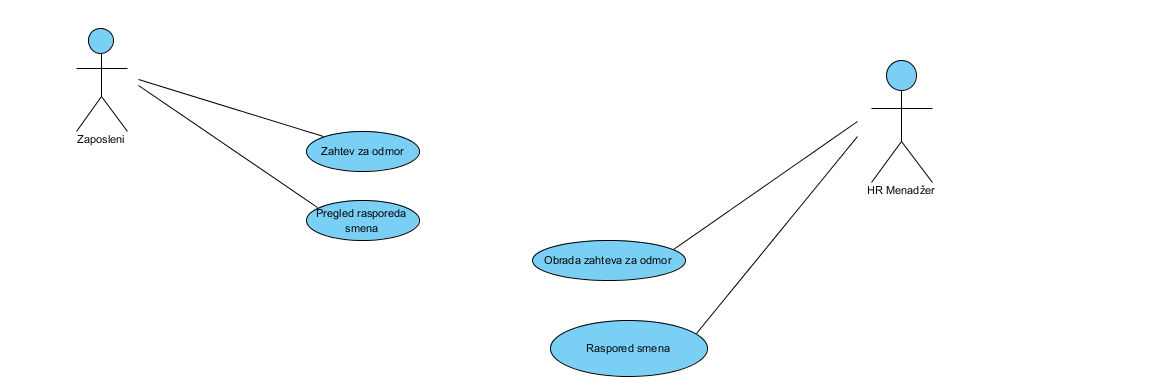
\includegraphics[width=\textwidth]{SU_4_hr.png}

\subsubsection{\textbf{Use Case}: Zahtev za odmor}
\textbf{Akter:} Radnik\\
\textbf{Ulaz:} Nema\\
\textbf{Izlaz:} Definisan zahtev za odmor\\
\textbf{Preduslovi:} Radnik poseduje username i lozinku za prijavljivanje na glavni sistem\\
\textbf{Postuslov:} Uspešno poslat zahtev za odmor\\
\textbf{Glavni tok:}
\begin{enumerate}
\item Radnik se prijavljuje na sistem.
\item Radnik bira segmet datuma za odmor.
\item Radnik potvrđuje izbor datuma, koji se nakon toga beleži u sistem i prosleđuje na dalju obradu.
\end{enumerate}
\textbf{Alternativni tokovi:} \\
\begin{itemize}
\item [1.1.] Prijavljivanje nije uspešno, korisnik se preusmerava na poruku sa greškom.
\item [2.1.] Uneti datumi nisu validni, korisnik se moli da ponovo unese datume i nastavlja ka 3. koraku
\end{itemize}

\subsubsection{\textbf{Use Case}: Obrada zahteva za odmor}
\textbf{Akter:} Menadžer\\
\textbf{Ulaz:} Spiskovi zahteva za odmor\\
\textbf{Izlaz:} Definisani odgovori na zahteve\\
\textbf{Preduslovi:} Menadžer se uspešno ulogovao na sistem i spiskovi zahteva su uspešno stigli do njega\\
\textbf{Postuslov:} Odgovori su definisani\\
\textbf{Glavni tok:}
\begin{enumerate}
\item Menadžer uzima spiskove za odmor
\item Za svakog radnika iz spiska, menadžer posebno gleda :
\begin{enumerate}[1.]
\item Da li radnik ima dovoljan broj preostalih slobodnih dana 
\item Da li je moguće organizovati funkcionisanje restorana u datom periodu bez dotičnog radnika
\end{enumerate}
\item Na osnovu procena stanja menadžer donosi odluku za svakog radnika pojedinačno.
\item Za svakog radnika pojedinačno, menadžer potvrđuje odgovor koji se dalje prosleđuje sistemu.
\end{enumerate}
\textbf{Alternativni tokovi:}\\
\begin{itemize}
\item[2.2.1.] Ukoliko su navedeni zahtevi za slobodnim danima definisani zakonom(slava, selidba, smrtni slučaj, ro]enje deteta,..) dani se odobravaju bez dodatnih procena i prelazi se na \textbf{3.} korak.
\end{itemize}

\subsubsection{\textbf{Use Case}: Raspored smena}
\textbf{Akter:} Menadžer\\
\textbf{Ulaz:} Nema\\
\textbf{Izlaz:} Novi raspored smena za određeni period\\
\textbf{Preduslovi:} Menadžer se uspešno ulogovao u sistem, postoje informacije o planu rada restorana za dati period kao i spisak godišnjih odmora\\
\textbf{Postuslov:} Sastavjen je novi raspored smena za određeni period i spreman je za slanje\\
\textbf{Glavni tok:} 
\begin{enumerate}
\item Menadžer definiše period za koji želi da napravi raspored smena
\item Menadžer proverava plan rada restorana u datom periodu
\item Menadžer proverava definisane godišnje odmore u datom periodu
\item Na osnovu informacija dobijenih iz koraka \textbf{2} i \textbf{3} menadžer pravi raspored smena
\end{enumerate}

\textbf{Alternativni tokovi:} \\
\begin{itemize}
\item [1.1.] Za dati period je već definisan raspored smena. Menadžer prelazi na korak 2 da bi menjao postojeći raspored.
\end{itemize}

\subsubsection{\textbf{Use Case}: Pregled rasporeda smena}
\textbf{Akter:} Radnik\\
\textbf{Ulaz:} Nema\\
\textbf{Izlaz:} Raspored smena za radnika\\
\textbf{Preduslovi:} Radnik poseduje username i lozinku za prijavljivanje na glavni sistem\\
\textbf{Postuslov:} Uspešan pregled smena\\
\textbf{Glavni tok:}
\begin{enumerate}
\item Radnik se prijavio na sistem.
\item Radnik unosi datum za koji želi da vidi svoj raspored smena.
\item Radnik ima na pregled raspored smena.
\end{enumerate}
\textbf{Alternativni tokovi:}\\
\begin{itemize}
\item [1.1.] Prijavljivanje nije uspešno, korisnik se preusmerava na poruku sa greškom.
\item [2.1.] Uneti datumi nisu validni, korisnik se moli da ponovo unese datume i nastavlja ka 3. koraku
\item[2.2.] Još nije definisan raspored smena za izabrani datum. Radnik se može vratiti na 2. korak , ili izlogovati sa sistema.
\end{itemize}

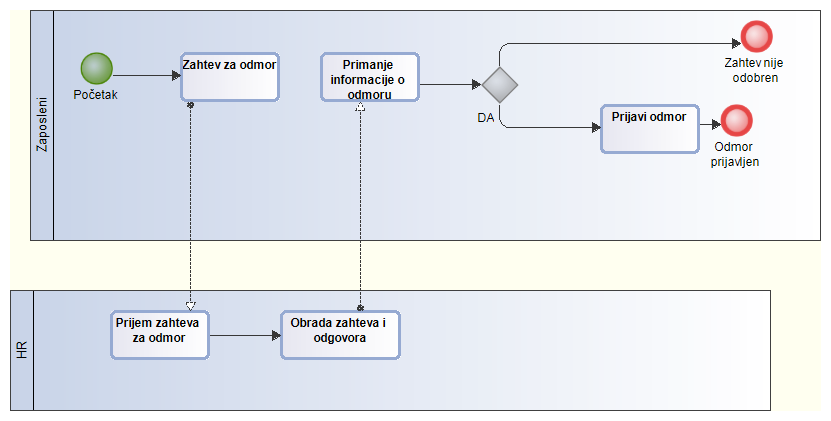
\includegraphics[width=\textwidth]{SU_4_Odmor.png}\\
\includegraphics[width=\textwidth]{SU_4_Raspored_smena.png}\\

%%%%%%%%%%%%%%%%%%%%%%%%%%%%%%%%%%%%%%%%%%%%%%%%%%%%%%%%%%%%%%%%%%%%%%%%%%%%

\subsection{Prihvatanje rezervacija gostiju}
\textbf{Prihvatanje rezervacija gostiju} je slučaj upotrebe u kojem se vrši prihvatanje i obrada digitalnih rezervacija mesta u restoranu. U tom procesu učestvuju potencijalni gost restorana, šef smene/sale restorana, kao i ostali zaposleni.\\

\begin{itemize}
\item Potencijalni gost restorana posećuje stranicu za digitalne rezervacije i unosi sve potrebne podatke za rezervaciju
\item Šef smene ili sale odobrava rezervaciju na osnovu pregleda prethodno unetih rezervacija i potvrdjuje(ili odbija) rezervaciju potencijalnom gostu.
\end{itemize}
\vspace{1cm}
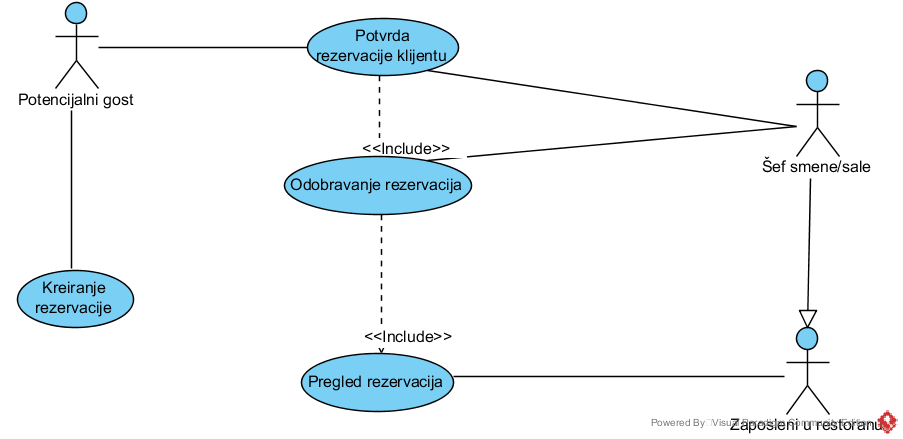
\includegraphics[width=\textwidth]{SU_5_prihvatanje_rezervacija.png}

\subsubsection{\textbf{Use Case}: Kreiranje rezervacije}
\textbf{Akter:} Potencijalni gost restorana (PG)\\
\textbf{Ulaz:} Kontakt podaci potencijalnog gosta (ime, prezime, kontakt telefon ili e-mail adresa), datum rezervacije, broj gostiju, specijalne napomene\\
\textbf{Izlaz:} Redni broj zahteva za rezervaciju.\\
\textbf{Preduslovi:} Nema.\\
\textbf{Postuslov:} Uspešno je kreiran zahtev za rezervaciju.\\
\textbf{Glavni tok:}
\begin{enumerate}
\item PG vrši navigaciju na stranu za rezervaciju
\item PG unosi zahtevane podatke
\item PG šalje restoranu zahtev za rezervaciju
\item PG dobija potvrdu da je zahtev za rezervaciju dostavljen restoranu na obradu.\\
\end{enumerate}
\textbf{Alternativni tokovi:}\\
\begin{itemize}
\item [4.1.]  Potvrda o poslatom zahtevu ne stiže u roku od 2 minuta
\item [4.1.1.]  Prikazuje se poruka sa izvinjenjem i kontakt telefonom kojim se rezervacija može izvršiti "offline".
\end{itemize}

\subsubsection{\textbf{Use Case}: Pregled rezervacija}
\textbf{Akter:} Zaposleni restorana\\
\textbf{Ulaz:} Datum i/ili broj stola za koji se pregleda spisak rezervacija.\\
\textbf{Izlaz:} Spisak registrovanih rezervacija koje odgovaraju kriterijumu pretrage.\\
\textbf{Preduslovi:} Zaposleni ima pristup glavnom sistemu.\\
\textbf{Postuslov:} Nema.\\
\textbf{Glavni tok:}
\begin{enumerate}
\item Korisnik se prijavljuje na sistem
\item Korisnik unosi ulazne parametre
\item Korisnik dobija tabelarni prikaz registrovanih rezervacija koje zadovoljavaju kriterijume pretrage.\\
\end{enumerate}
\textbf{Alternativni tokovi:}\\
        1.1. Prijavljivanje nije uspešno, korisnik se preusmerava na poruku sa greškom.\\

\subsubsection{\textbf{Use Case}:  Odobravanje rezervacija}
\textbf{Akter:} Šef smene/sale\\
\textbf{Ulaz:} Podaci iz pristiglog zahteva za rezervaciju, informacije o već registrovanim rezervacijama i raspoloživom broju i strukturi mesta.\\
\textbf{Izlaz:} Rezervacija odobrena ili odbijena i redni broj rezervacije.\\
\textbf{Preduslovi:} Postoji barem jedan neobrađen zahtev za rezervaciju i trenutni korisnik sistema ima pravo da pristupi odobravanju rezervacija.\\
\textbf{Postuslov:} Informacije o odobrenim rezervacijama su sačuvane u sistemu.\\
\textbf{Glavni tok:}
\begin{enumerate}
\item Korisnik se prijavljuje na sistem
\item Korisnik pregleda spisak dospelih zahteva za rezervaciju
\item Korisnik za svaki od zahteva vrši pregled rezervacija da bi utvrdio da li je rezervacija sa zadatim parametrima moguća
\item Korisnik odobrava ili odbija rezervaciju i svoju odluku registruje u sistemu.\\
\end{enumerate}
\textbf{Alternativni tokovi:}\\
\begin{itemize}
\item [1.1.] Prijavljivanje nije uspešno, korisnik se preusmerava na poruku sa greškom.
\end{itemize}

\subsubsection{\textbf{Use Case}: Uklanjanje registrovanih rezervacija}
\textbf{Akter:} Šef smene/sale\\
\textbf{Ulaz:} Redni broj rezervacija koju treba obrisati i razlog brisanja.\\
\textbf{Izlaz:} Nema.\\
\textbf{Preduslovi:} Trenutni korisnik ima pravo da pristupi meniju za uklanjanje registrovanih rezervacija. Postoji validan razlog za uklanjanje rezervacije koji je iskomuniciran sa klijentom (sa čije god strane da je razlog potekao).\\
\textbf{Postuslov:} Rezervacija sa datim rednim brojem je uklonjena iz sistema i razlog uklanjanja je registrovan.\\
\textbf{Glavni tok:}
\begin{enumerate}
\item Korisnik se prijavljuje na sistem
\item Korisnik unosi ulazne podatke
\item Rezervacija se uklanja iz sistema
\item Korisniku se prikazuju preostale rezervacije za dan uklonjene rezervacije.\\
\end{enumerate}
\textbf{Alternativni tokovi:}\\
\begin{itemize}
\item [1.1.] Prijavljivanje nije uspešno, korisnik se preusmerava na poruku sa greškom.
\item [3.1.] Rezervacija sa datim rednim brojem ne postoji u sistemu. Korisniku se prijavljuje greška i prikazuje se spisak poslednjih deset uklonjenih rezervacija.
\end{itemize}

\subsubsection{\textbf{Use Case}: Potvrda rezervacije klijentu}
\textbf{Akter:} Šef smene/sale, potencijalni gost restorana.\\
\textbf{Ulaz:} Redni broj rezervacije i kontakt podaci potencijalnog gosta.\\
\textbf{Izlaz:} Rezervacija je potvrdjena ili ne.\\
\textbf{Preduslovi:} Trenutni korisnik ima pravo da pristupi meniju za potvrdjivanje rezervacija, kontakt podaci potencijalnog gosta su validni.\\
\textbf{Postuslov:} Rezervacija je potvrdjena.\\
\textbf{Glavni tok:}
\begin{enumerate}
\item Korisnik se prijavljuje na sistem
\item Korisnik pregleda odabranu rezervaciju
\item Korisnik šalje potvrdu gostu automatski generisanom elektronskom poštom ili poziva gosta telefonom.\\
\end{enumerate}
\textbf{Alternativni tokovi:}\\
\begin{itemize}
\item [1.1.] Prijavljivanje nije uspešno, korisnik se preusmerava na poruku sa greškom.
\item [3.1.] Kontakt podaci nisu validni, rezervacija se automatski registruje kao uklonjena, sa razlogom "nevalidni kontakt podaci gosta".
\end{itemize}
  
%%%%%%%%%%%%%%%%%%%%%%%%%%%%%%%%%%%%%%%%%%%%%%%%%%%%%%%%%%%%%%%%%%%%%%%%%%%%

\subsection{Online naručivanje i dostava hrane i pića}
Online naručivanje i dostava hrane i pića je slučaj upotrebe gde mušterija definiše svoju narudžbinu, radnici je prave, a dostavljači isporučuju. U naručivaju učestvuju: mušterija, radnik i dostavljač.
\\
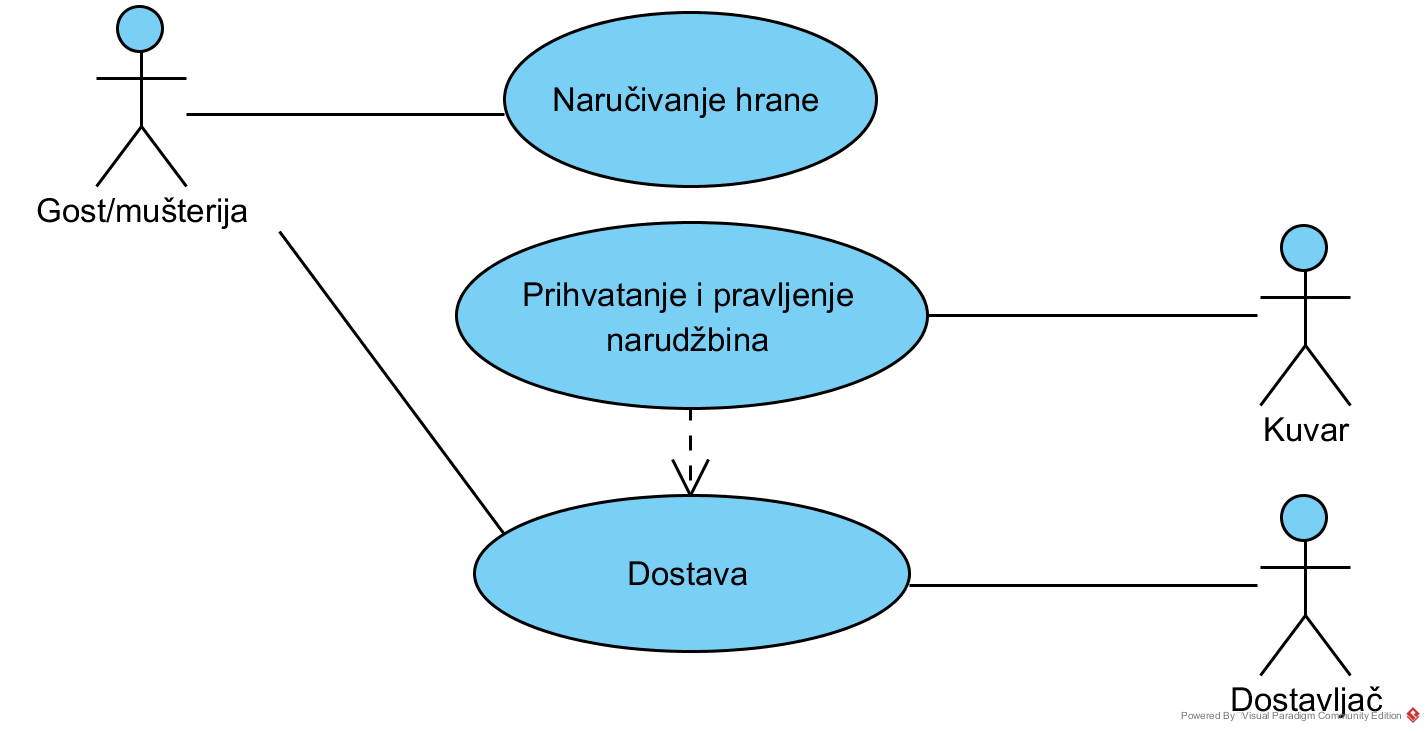
\includegraphics[width=\linewidth]{SU_6_dostava.png}

\subsubsection{\textbf{Use Case}: Pravljenje narudžbine}
\textbf{Akter:} Mušterija\\
\textbf{Ulaz:} Kontakt podaci mušterije (ime, prezime, kontakt telefon ili e-mail adresa), datum rezervacije, broj gostiju, specijalne napomene\\
\textbf{Izlaz:} Definisana narudžbina\\
\textbf{Preduslovi:} Restoran prima narudžbine\\
\textbf{Postuslov:} Uspešno napravljena narudžbina je poslata restoranu\\
\textbf{Glavni tok:}
\begin{enumerate}
\item Mušterija vrši odabir hrane i pića
\item Mušerija potvrđuje narudžbinu
\item Korisnik dobija potvrdu da je narudžbina dostavljena restoranu na obradu.\\
\end{enumerate}
\textbf{Alternativni tokovi:} \\
\begin{itemize}
\item [3.1.] Potvrda o poslatom zahtevu ne stiže u roku od 2 minuta
\item [3.1.1.] Prikazuje se poruka sa izvinjenjem i kontakt telefonom kojim se narudžbina može izvršiti "offline".
\end{itemize}


\subsubsection{\textbf{Use Case}: Prihvatanje i pravljenje narudžbina}
\textbf{Akter:} Radnik, Dostavljač\\
\textbf{Ulaz:} Spisak narudžbina\\
\textbf{Izlaz:} Napravljene narudžbine\\
\textbf{Preduslovi:} Radnik se uspešno ulogovao na sistem i spiskovi narudžbina su uspešno stigli do njega\\
\textbf{Postuslov:}  Napravljene narudžbine su spremne za dostavu\\
\textbf{Glavni tok:}
\begin{enumerate}
\item Radnik uzima spiskove narudžbina.
\item Za svaku narudžbinu iz spiska pravi se porcija, po redosledu vremena naručivanja.
\item Po završetku pravljenja obroka, radnik obaveštava Dostavljača da je porudžbina spremna za dostavu 
\end{enumerate}
\textbf{Alternativni tokovi:}\\
\begin{itemize}
\item [2.1.] Ukoliko  fale sastojci za neku od narudžbina, prelazi se na sledeću narudžbinu dok sastojci ne stignu
\end{itemize}
       
       
\subsubsection{\textbf{Use Case}: Dostava i prihvatanje dostave}
\textbf{Akter:} Dostavljač, Mušterija\\
\textbf{Ulaz:} Pripremljena narudžbina\\
\textbf{Izlaz:} Izvršena dostava\\
\textbf{Preduslovi:} Mušterija je ispravno definisala adresu\\
\textbf{Postuslov:}  Izvršena dostava je plaćena\\
\textbf{Glavni tok:}
\begin{enumerate}
\item Dostavljač odnosi porudžbina na adresu definisanu na narudžbini
\item Mušterija prihvata porudžbinu i proverava da li je sve u redu sa sadržajem
\item Mušterija plaća dostavu
\end{enumerate}
\textbf{Alternativni tokovi:}\\
\begin{itemize}
\item [2.1.]  Ukoliko nije sve u redu sa sadržajem, pravi se nova narudžbna i mušterija čeka novu dostavu, ili mušterija odustaje od narudžbine.
\item [2.1.1] Ukoliko je mušterija odustala, dostavljač vraća hranu u restoran.
\end{itemize}

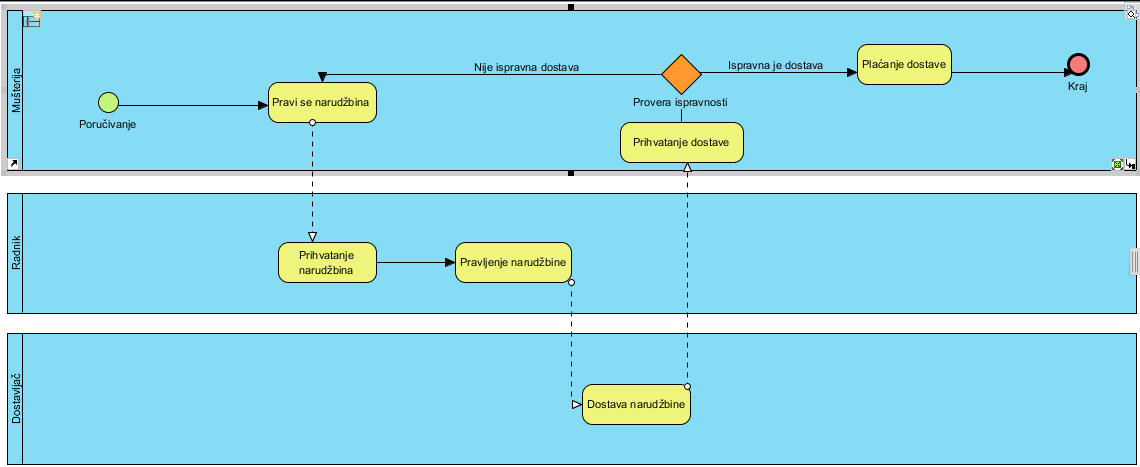
\includegraphics[width=\textwidth]{SU_6_dostava_bpmn.png}

%%%%%%%%%%%%%%%%%%%%%%%%%%%%%%%%%%%%%%%%%%%%%%%%%%%%%%%%%%%%%%%%%%%%%%%%%%%%
\subsection{Obrada porudžbine gosta}
\subsubsection{\textbf{Use Case}: Gost poručuje jelo}
\textbf{Akteri:} Gost kafane, konobar\\
\textbf{Ulaz:} Jelovnik.\\
\textbf{Izlaz:} Porudžbina.\\
\textbf{Preduslov:} Gost je u kafani.\\
\textbf{Postuslov:} Uspešno je napravljen skup porudžbina gosta.\\
\textbf{Glavni tok:}
\begin{enumerate}
\item Gost potražuje jelo sa menija
\item Konobar uspešno beleži narudžbinu \\
\end{enumerate}
\textbf{Alternativni tokovi:} \

\subsubsection{\textbf{Use Case:} Konobar prenosi porudžbinu kuhinji}
\textbf{Akteri:} Konobar\\
\textbf{Ulaz:} Jelovnik\\
\textbf{Izlaz:} Osvežen globalni spisak porudžbina kojim se vodi rad kuhinje\\
\textbf{Preduslov:} Konobar je preuzeo porudžbinu od gosta.\\
\textbf{Postuslov:} Porudžbina je sačuvana na sigurnom mestu gde će biti preuzeta od strane kuhinje.\\
\textbf{Glavni tok:}
\begin{enumerate}
\item Konobar dodaje porudžbinu na listu porudžbina.
\end{enumerate}
\textbf{Alternativni tokovi:}
\begin{enumerate}
\item Konobar ne uspeva da doda porudžbinu usred tehničkih problema sistema, pa lično prenosi porudžbinu kuhinji.
\end{enumerate}

\subsubsection{\textbf{Use Case:} Kuhinja obrađuje porudžbinu}
\textbf{Akteri:} Kuhinja (kuvar), konobar\\
\textbf{Ulaz:} Porudžbina sa globalne liste porudžbina\\
\textbf{Izlaz:} Pripremljeno jelo sa porudžbine.\\
\textbf{Preduslov:} Postoji bar jedna porudžbina na listi\\
\textbf{Postuslov:} Pripremljena sva jela sa odabrane porudžbine\\
\textbf{Glavni tok:}
\begin{enumerate}
\item Kuvar bira najstariju porudžbinu (onu koja je najduže čekala da bude obrađena).
\item Kuvar sprema jela sa porudžbine.
\item Nakon pripreme jela, kuhinja kontaktira konobara da preuzme jelo, i odnese ga gostu.
\end{enumerate}
\textbf{Alternativni tokovi:}
\begin{enumerate}
\item [2.1.] Nema svih sastojaka potrebnih za pripremu jela.
\item [2.1.1.] Kuvar naručuje potrebne sastojke, ukoliko ne mogu da stignu u određenom vremenskom periodu, kontaktira se konobar da pita mušteriju za drugi odabir. 
\end{enumerate} Nema svih sastojaka potrebnih za pripremu jela.\\

 
 
\subsubsection{\textbf{Use Case:} Isporuka jela}
\textbf{Akteri:} Konobar, gost\\
 \textbf{Ulaz:} Gotovo jelo koje je konobar preuzeo iz kuhinje\\
 \textbf{Izlaz:} Servirano jelo na stolu gosta kafane.\\
 \textbf{Preduslov:} Kuhinja pripremila jelo\\
 \textbf{Postuslov:} Gost jede jelo.\\
 \textbf{Glavni tok:} 
\begin{enumerate}
\item Kuhinja obaveštava konobara da su sva jela sa odredjene narudžbine pripremljena.
\item Konobar preuzima jelo, i odnosi ga do gosta čija narudžbina je obradjena. 
\end{enumerate}
\textbf{Alternativni tokovi:} \\
\subsubsection{\textbf{Use Case:} Online narudžbina}
\textbf{Akteri:} Posetilac sajta\\
\textbf{Ulaz:} Online ponuda jela\\
\textbf{Izlaz:} Online porudžbina\\
\textbf{Preduslov:} Posetilac sajta ima stabilnu internet konekciju.\\
\textbf{Postuslov:} Porudžbina je upisana u globalni spisak porudžbina kojim se vodi rad kuhinje\\
\textbf{Glavni tok:} Klijent posećuje sajt, i bira jelo koje želi da naruči.\\
\textbf{Alternativni tok:} Porudžbina nije prihvaćena (usled gužve u kuhinji, problema sa konekcijom sa klijentom ili nekog drugog razloga)\\
  
  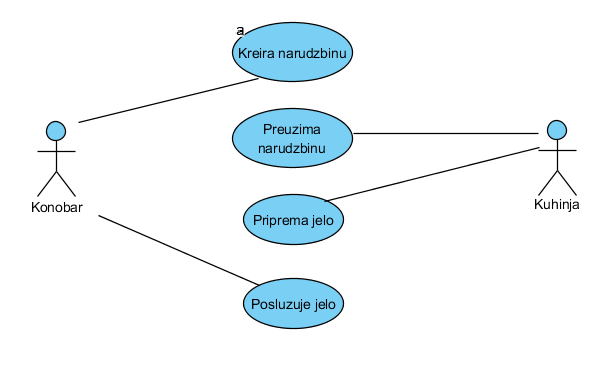
\includegraphics[width=\textwidth]{SU_7_konobar_kuhinja.png}
  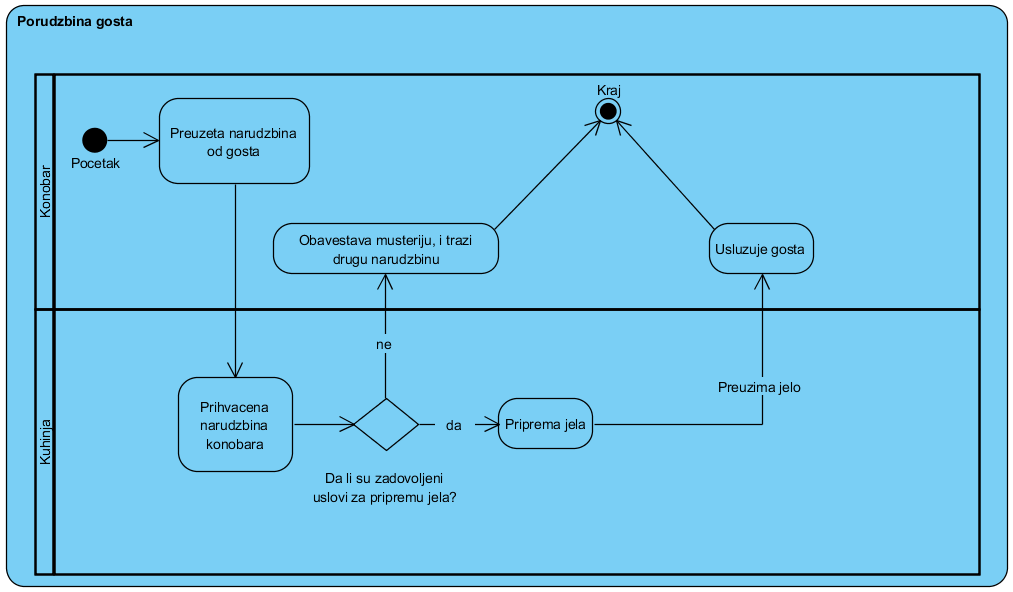
\includegraphics[width=\textwidth]{SU_7_porudzbina.png}


%%%%%%%%%%%%%%%%%%%%%%%%%%%%%%%%%%%%%%%%%%%%%%%%%%%%%%%%%%%%%%%%%%%%%%%%%%%%

\section{Baza podataka}
 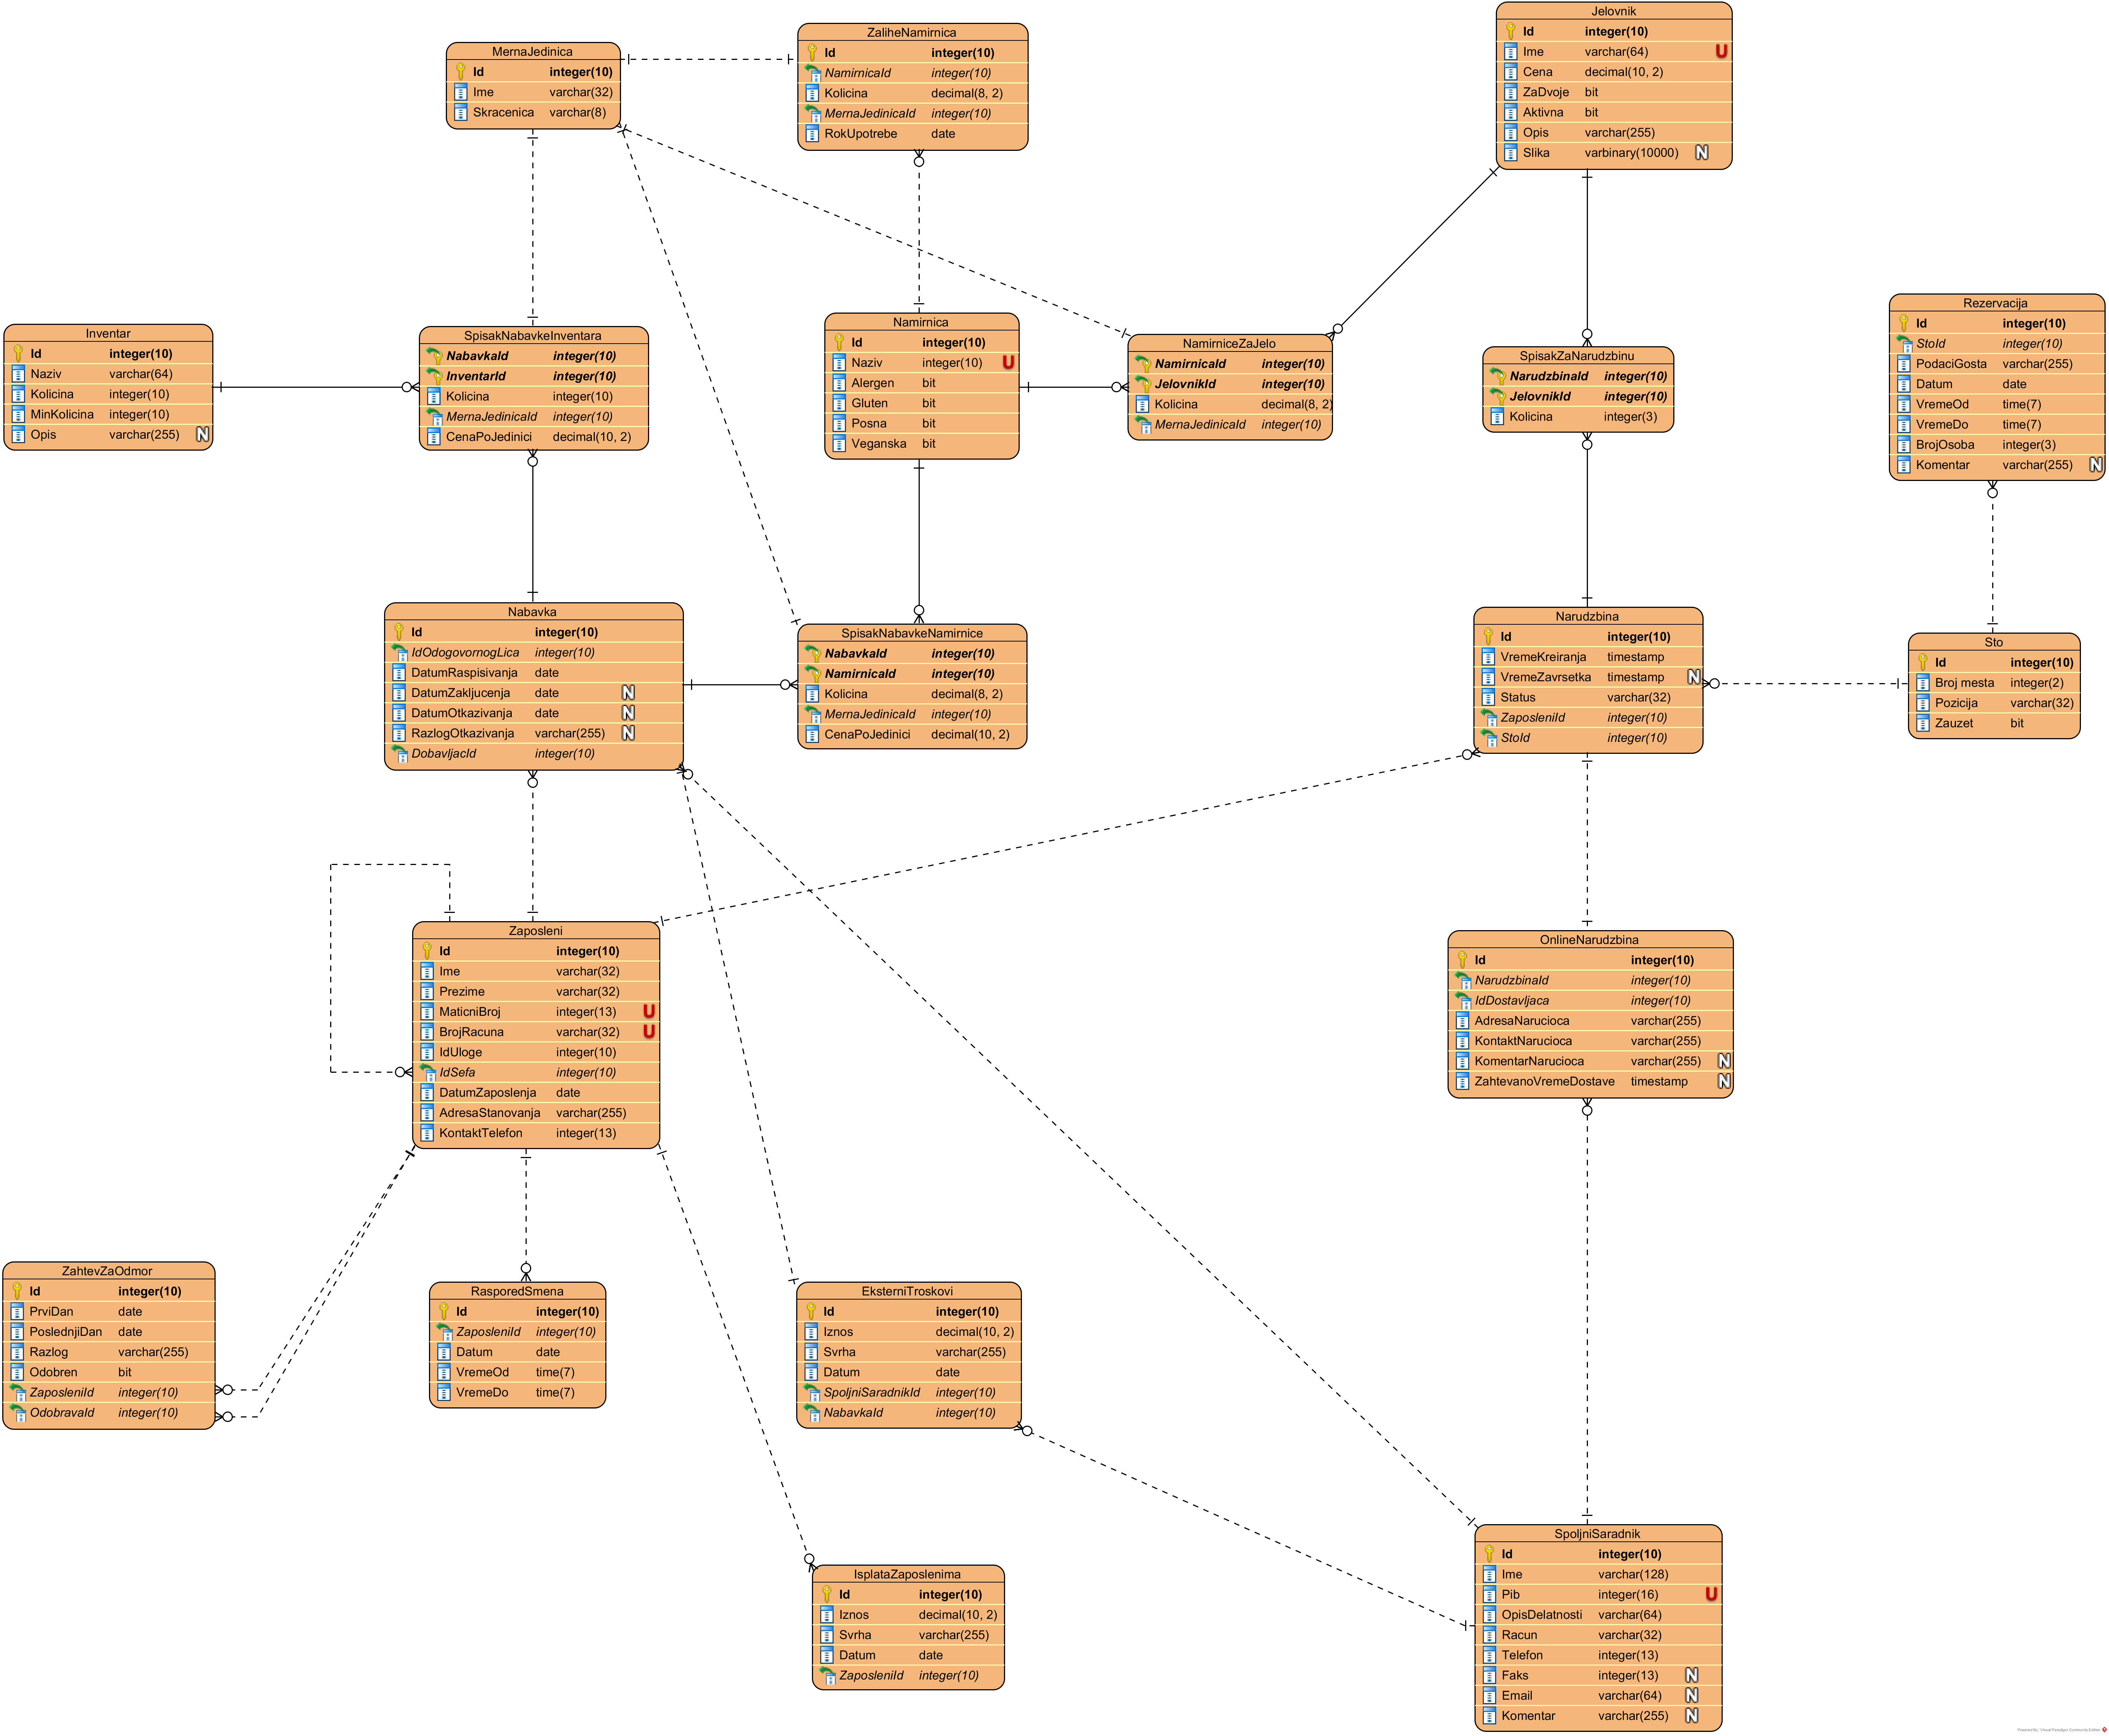
\includegraphics[width=\textwidth]{NajmanjiProblem_BazaPodataka.png}
 
 
\textbf{Kreiranje trebovanja} :
\begin{itemize}
\item Novi red u \emph{Nabavka}
\item Za svaku stavku koja se traži, dodaje se novi red u \emph{SpisakNabavkeInventara} sa predmetom i količnom
\item Ako novi predmet nije postojao, dodaje se i novi red u \emph{Inventar}, gde je default vrednost za \emph{Kolicinu} 0, a \emph{MinKolicina} se postavlja rucno
\end{itemize}


\textbf{Pregled stanja inventara} :
\begin{itemize}
\item Pregled tabele \emph{Inventar}. Zahteva se primarni indeks na id koloni zbog joinova i na naziv radi lake pretrage po nazivu (nonclustered)
\item Druga varijanta, pregled view-a \emph{InventarNaIzmaku} koji sadrži samo one stavke koje su jako blizu ili ispod granice \emph{MinKolicina} za funkcionisanje
\end{itemize}

\textbf{Unošnje proizvoda u sistem:}
\begin{itemize}
\item Unošenje novog reda u tabelu \emph{Inventar}, sa količinom jednakom nuli po default. Mora postojati dokaz o nabavci, tako da veličina veca od nule za početnu vrednost ne bi trebalo da ima smisla
\end{itemize}

\textbf{Pristizanje inventara}
\begin{itemize}
\item Pregleda se spisak \emph{Nabavka x SpisakNabavkeInventara}, i poziva se stored procedura koja validira nabavku, unosi \emph{DatumPristizanja}, povećava količinu za svaku pogođenu stavku inventara 
\end{itemize}

\textbf{Kreiranje liste zaliha na minimumu}
\begin{itemize}
\item Pregled odgovarajućeg pogleda \emph{ZaliheNaIsteku} koji oslikava to stanje 
\end{itemize}


\textbf{Unos namirnica u sistem}
\begin{itemize}
\item Unos novog reda u tabelu \emph{Namirnice} sa potrebnim podacima 
\end{itemize}

\textbf{Kreiranje porudžbine}
\begin{itemize}
\item Dodavanje novog reda u tabelu \emph{Nabavka} i potrebnih redova u tabelu \emph{SpisakNabavkeNamirnice}
\end{itemize}

\textbf{Pristizanje namirnica}
\begin{itemize}
\item Poziv odgovarajuće stored procedure koja upisuje datum zaključenja nabavke, ažuriranje tabele \textbf{Zalihe} namirnica sa ručnim unošenjem roka upotrebe unetih artikala 
\end{itemize}

\textbf{Ažuriranje jelovnika}
\begin{itemize}
\item Vrši se automatski postavljanjem oznake omogućeno/onemogćeno od strane odgovarajućeg trigera nakon svakog uklanjanja namirnice sa stanja zaliha odnosno nakon unosa namirnica u sistem
\end{itemize}


-------------------------------

\textbf{Obrada zahteva za odmor}
\begin{itemize}
\item U odgovarajućem zahtevu za odmor se menja flag odobren
\item Aktivira se triger koji u rasporedu smena uklanja radnika iz rasporeda u periodu kada je na odmoru
\end{itemize}

\textbf{Zahtev za odmor}
\begin{itemize}
\item Vrši se insert novog reda u tabelu \emph{ZahtevZaOdmor} 
\end{itemize}

\textbf{Raspored smena}
\begin{itemize}
\item Za dati datum se unosi po jedan red za svakog zaposlenog, za svaki kontinualni segment rada. Odgovarajućom stored procedurom se može ponoviti raspored i za sledeći dan
\end{itemize}

\textbf{Pregled rasporeda smena}
\begin{itemize}
\item Vrši se pregled tabele raspored smena, tako što se za vrednosti koje nisu pokrivene nijednim unosom smatra da niko nije raspoređen
\end{itemize}


\textbf{Kreira narudžbinu}
\begin{itemize}
\item Unosi se novi red za svaki sto koji je zahvaćen narudžbinom i pravi se odgovarajući spisak za narudžbinu
\end{itemize}


\textbf{Preuzima narudžbinu}
\begin{itemize}
\item Menja se status narudžbine 
\end{itemize}

\textbf{Poslužuje jelo}
\begin{itemize}
\item Menja status narudžbine i registruje njen završetak
\item Pri uklanjanju pribora sa stola, sto se markira kao slobodan
\end{itemize}


\textbf{Priprema jela}
\begin{itemize}
\item Nakon što je priprema gotova, menja se status narudžbine na odgovarajući način
\end{itemize}


\textbf{Naručivanje hrane}
\begin{itemize}
\item Kreiranje online narudžbine unosi novi red u \emph{OnlineNarudzbina}. To dalje kreira narudžbinu kao i u prethodnom slučaju.
\end{itemize}

\textbf{Prihvatanje i pravljenje narudžbina}
\begin{itemize}
\item Isto kao za preuzimanje narudžbina, pošto je tabela \emph{Naruzdbina} ono sto kuhinja zapravo vidi
\end{itemize}


\textbf{Dostava}
\begin{itemize}
\item Menja se status narudzbine na odgovarajući kada dostavljač potvrdi dostavu
\end{itemize}

\textbf{Kreiranje rezervacija}
\begin{itemize}
\item  Dodaje se novi red u tabelu rezervacija ukoliko je to moguće zbog ograničenja 
\end{itemize}


\textbf{Pregled rezervacija}
\begin{itemize}
\item Vrši se pregled tabele za rezervacije 
\end{itemize}


\textbf{Odobravanje rezervacija}
\begin{itemize}
\item Dodeljuje se NOT NULL vrednost za StoId 
\end{itemize}

\textbf{Potvrda rezervacije}
\begin{itemize}
\item Menjaju se podaci ukoliko je potrebno. Ukoliko nema uspešne potvrde, rezervacija se briše iz sistema.
\end{itemize}

\textbf{Pregled finansija restorana za traženi period}
\begin{itemize}
\item  Podaci se dobijaju iz odgovarajućeg pogleda, koji objedinjuje podatke iz spiska odliva zbog nabavki (a preko \emph{SpiskaNabavkiNamirnica} i \emph{SpiskaNabavkeInventara} ), materijalnih troskova (\emph{IsplataZaposlenima} i \emph{EksterniTroskovi}) kao i priliva na osnovu podataka povezanih sa narudžbinama 
\end{itemize}

\textbf{Štampanje finansijskog izvestaja za trazeni period}
\begin{itemize}
\item Nema aktivnosti po bazi osim pregleda kao u prethodnoj stavci 
\end{itemize}

\textbf{Pregled najčešćih/najređih narudžbina}
\begin{itemize}
\item Podaci se dobijaju iz odgovarajućeg pogleda, na osnovu podataka iz tabele \emph{Narudžbina} i sa njom povezanih spiskova.
\end{itemize}

%%%%%%%%%%%%%%%%%%%%%%%%%%%%%%%%%%%%%%%%%%%%%%%%%%%%%%%%%%%%%%%%%%%%%%%%%%%%

\section{Predlog korisničkog interfejsa}

%% cekamo implementaciju za skice
%%%%%%%%%%%%%%%%%%%%%%%%%%%%%%%%%%%%%%%%%%%%%%%%%%%%%%%%%%%%%%%%%%%%%%%%%%%%

\section{Prototip}
%% cekamo implementaciju za opis
%%%%%%%%%%%%%%%%%%%%%%%%%%%%%%%%%%%%%%%%%%%%%%%%%%%%%%%%%%%%%%%%%%%%%%%%%%%%

\end{document}
